%!TEX root = ../../dissertation.tex
%%%%%%%%%%%%%%%%%%%%%%%%%%%%%%%%%%%%%%%%%%%%%%%%%%%%%%%%%%%%%%%%%%%%%%%%%%%%%%%%


%%%%%%%%%%%%%%%%%%%%%%%%%%%%%%%%%%%%%%%%%%%%%%%%%%%%%%%%%%%%%%%%%%%%%%%%%%%%%%%%
\section{Enhanced Mobile Measurement Approaches}
\label{c5:sec:mobilestreaming-measurements}


\gls{LTE}-\gls{EPC} Network Simulator (LENA)\cite{ns3lte}

Planetlab: an overlay testbed for broad-coverage services \cite{chun2003planetlab}

OsmocomBB project \cite{osmocombbwww}

Simulating LTE Cellular Systems: An Open-Source Framework \cite{5634134}



An evaluation of dynamic adaptive streaming over \gls{HTTP} in vehicular environments \cite{Muller:2012:EDA:2151677.2151686}


additional sensibility link-dump




%%%%%%%%%%%%%%%%%%%%%%%%%%%%%%%%%%%%%%%%%%%%%%%%%%%%%%%%%%%%%%%%%%%%%%%%%%%%%%%%
\subsection{Enriching Mobile Measurements with Additional Metadata}
\label{c5:sensorium}

Seattle Testbed

Sensibility Testbed (https://sensibilitytestbed.com/projects/project): Followup-Project to Sensorium, building entirely on Seattle/Python


\subsubsection{Preserving Privacy}

critical element for acceptance of an active network measurement mobile app is to preserve the privacy of the participating users. This is especially true for free-form network testbeds, that allow running arbitrary experiments or even code. Access to sensitive data has to be regulated, filtered, adjusted, or even outright prevented. Even more concerning (for privacy reasons) but also raising hope (for scientific experimentation) is the steadily rising number of sensors in mobile devices. Nowadays included are even heartbeat monitors and fingerprint sensors. The future may hold even more medical and body-related sensors revealing many private details on their users.

Android AppOps

https://guardianproject.info/

CyanogenMod Privacy Guard (https://plus.google.com/+CyanogenMod/posts/gk7X3HjNvnH)

Software abstractions for trusted sensors \cite{Liu:2012:SAT:2307636.2307670}

TaintDroid: An Information-Flow Tracking System for Realtime Privacy Monitoring on Smartphones. \cite{enck2010taintdroid}

Dr. Android and Mr. Hide: Fine-grained Permissions in Android Applications \cite{Jeon:2012:DAM:2381934.2381938}

Improving wireless network performance using sensor hints \cite{ravindranath2011improving}

http://campar.in.tum.de/Chair/KalmanFilter

https://dsp.stackexchange.com/questions/320/is-a-kalman-filter-suitable-to-filter-projected-points-positions-given-euler-an/321\#321

SENSORIUM EXCURSION
CONTEXT: (active) measurements in mobile networks should make use of the device's current state and environment. i.e., read its sensor data and put measurements in context with it. Alternatively, use anonymized sensor data for new kinds of evaluations (can this device watch video at all at the current location?)
CONTEXT

Modern computing devices such as smartphones, laptops, and tablet computers are equipped with an increasing number of sensors: \gls{GPS}, tilt, and acceleration meters quantify the physical position and orientation of the device; 3G, WiFi, and other  interfaces gather data on the availability and signal quality of wireless networks; temperature and ambient light sensors deliver additional insight into a user's work and home environments.

There exist problems for the practical viability of collection data though: Different devices and platforms such as Android and iOS use very different interfaces into their sensors; privacy is another issue hardly tackled on any platform other than in a crude binary (allow/deny access) way. Therefore, in this demo we introduce Sensorium, a generic sensor reading framework that funnels data from actual sensor drivers, implements fine-grained privacy control for the user, and provides generic outbound interfaces such as \acrshort{XML}-\acrshort{RPC}. We also show an application using it, O3GM, which visualizes mobile coverage data coming from Sensorium.

%Sensor interfaces differ -> difficult to do generic stuff with them
Sensorium can access all the information a device provides and makes them available to other applications. Up until now, it has been a challenging task for software developers (especially scientists and experimenters) to implement specialized sensor applications. This task is simplified by providing a generic framework for interfacing sensors. In our current implementation, available for Android, most of the typical sensors are already implemented. Since giving access to sensor data also exposes the user's privacy, the user can disable or set privacy levels for each sensor individually, and all sensor readings that would be shared are displayed. %Setting higher privacy levels reduces the amount of data a sensor shares. %E.g., location data accuracy could be rounded, or just hashes of data shared.
\\

O3GM\footnote{\url{http://homepage.univie.ac.at/albert.rafetseder/o3gm}} showcases the sensors framework. It comprises a web service displaying cellular access technology data points at their \gls{GPS} locations collected by devices running Sensorium (see Figure~\ref{c5:fig:ogggm}). This solves a real-world problem: Currently, this kind of data is only available to mobile operators, which however  are hindered by commercial interests to make them publicly available --- at least in raw, unadorned form. Other projects such as OpenSignalMaps\footnote{\url{http://opensignal.com/}} and Sensorly\footnote{\url{http://www.sensorly.com/}}, as well as corporations like Google and Apple collect these data, but are very restrictive regarding usage by other parties. This is not true for O3GM:\@ We make the data points collected available as Open Data under an open content license.

Obviously, other applications are possible. Since code and data are open-sourced, everyone can implement their great ideas, port Sensorium to other platforms or reimplement our interface there, etc.

\begin{figure}[htb]
\centering
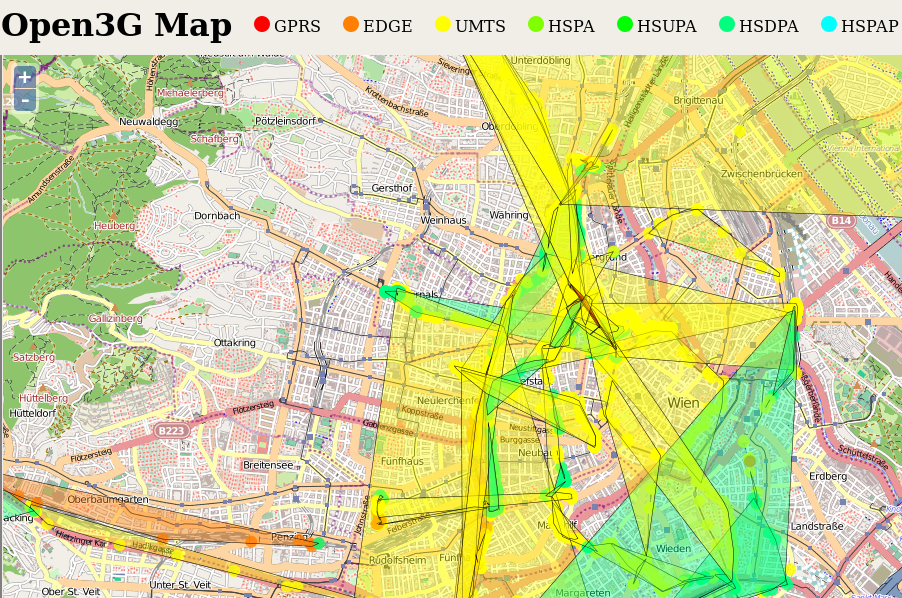
\includegraphics[width=\textwidth]{images/map-cells.png}
\caption{The O3GM web page, displaying \gls{3G} coverage measurements extracted from Sensorium on top of OpenStreetMap.}
\label{c5:fig:ogggm}
\end{figure}

\subsubsection{Architecture}

Figure~\ref{c5:fig:architecture} overviews Sensorium's architecture components, and its interplay with the data collecting parts of O3GM. \textit{Sensor drivers} are implemented on top of the operating system taking care of reading sensor values from platform-specific interfaces and pushing them upwards into the \textit{registry}. Here, sensor data is timestamped and collected. On one side, data are prepared for local display, e.g. in a \gls{GUI} or status widget. On the other side, a user-configurable \textit{privacy layer} might allow for full sensor access from above or reduce the precision of values (e.g. round \gls{GPS} coordinates); it could salt and hash sensor values for improved privacy, or completely deny access to individual (or all) sensors. Finally, other applications running on the same device are free to connect to Sensorium's \textit{outbound interfaces} to register for sensor updates or poll data. Access from sources other than localhost is not allowed for obvious privacy reasons.

Due to the layered architecture, it is very simple for contributors to add their own implementations of layers or swap them out for their own altogether. Consider a scenario when a contributor wishes to include a sensor we do not yet provide a driver for. All that needs to be implemented is code interfacing the actual sensor, and the lightweight API into our sensor registry. Similarly, additional local display methods, privacy enhancements, and outbound interfaces might be implemented.

\begin{figure}[htb]
\centering
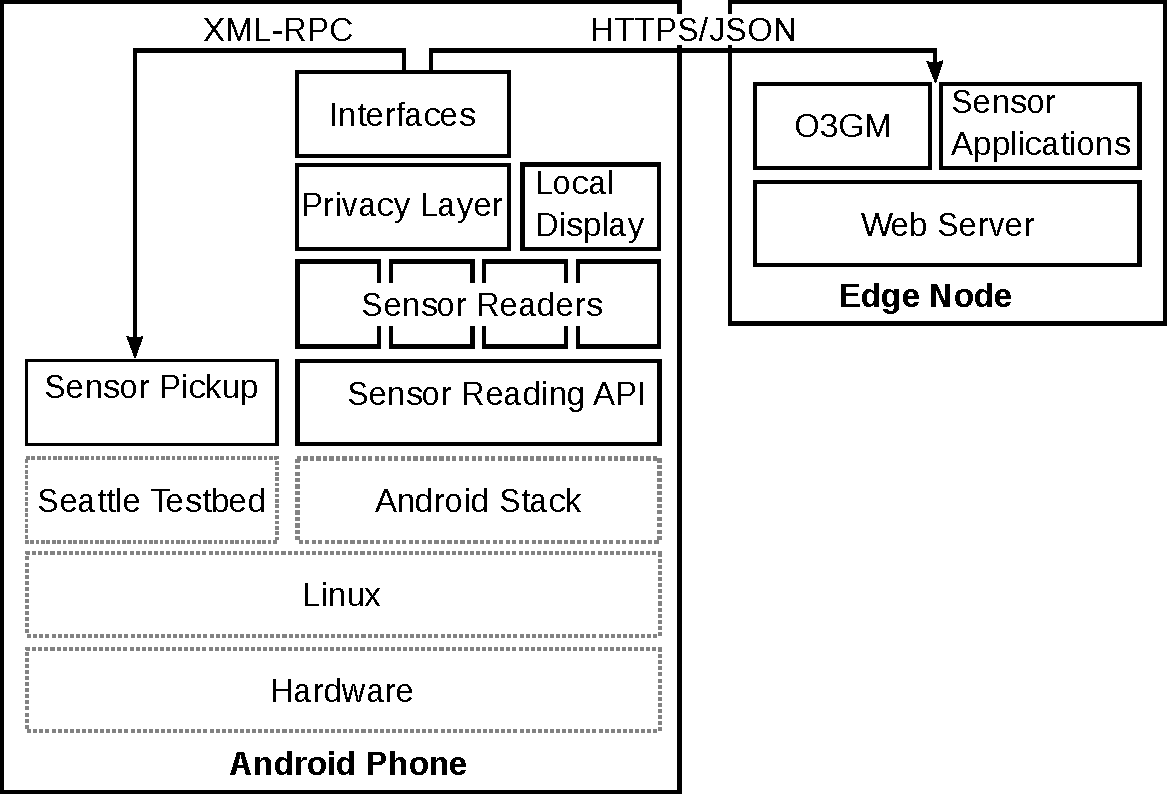
\includegraphics[width=0.9\textwidth]{images/sensorium-arch.pdf}
\caption{Sensorium architecture with O3GM \textit{pickup}~and \textit{server}. Components described in this paper are shown dark gray.}
\label{c5:fig:architecture}
\end{figure}

\subsubsection{Implementation}

Our current implementation of Sensorium\footnote{\url{https://github.com/fmetzger/android-sensorium}} runs on the Android platform. To provide a unified interface for accessing the sensor data we incorporated an \acrshort{XML}-\acrshort{RPC} library\footnote{\url{https://code.google.com/p/android-xmlrpc/}} that listens for connections on localhost, meaning that only applications running on the same device can access it. The pickup code\footnote{\url{https://homepage.univie.ac.at/albert.rafetseder/o3gm_pickup.repy}} to collect sensor values runs on top of the renowned Seattle\footnote{\url{https://seattle.cs.washington.edu/}} platform, which is also available for Android, and allows us to remotely and securely access the collected data, and easily experiment with energy and cost efficient data upload/download strategies. The example application we implemented to make use of Sensorium, O3GM\footnote{\url{https://github.com/lukpueh/Open3GMap}}, is based on JavaScript and the OpenLayers\footnote{\url{http://openlayers.org/}} library. All of our code is dual-licensed under \gls{GPLv3} and the \acrshort{BSD} license.

\begin{figure}[htb]
\centering
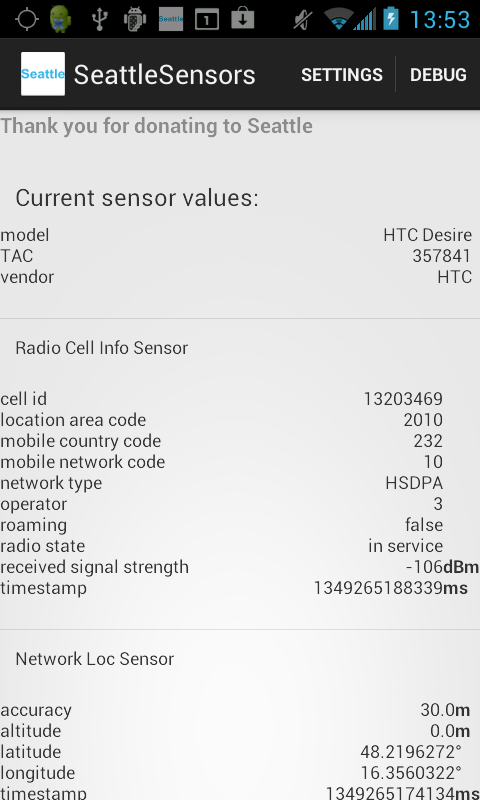
\includegraphics[width=0.45\textwidth]{images/sesescreenshot.png}
\caption{Sensorium screenshot.}
\label{c5:fig:screenshot}
\end{figure}

Sensorium consists of a base registry service with a common interface which each sensor implementation can easily be plugged into. All values are also displayed for the user as seen in Figure~\ref{c5:fig:screenshot}. The privacy layer automatically anonymizes all gathered values before making them available through XML-RPC in accordance with the user's current privacy settings.

We currently provide sensor implementations for generic device information, e.g. device name and battery status; mobile radio data such as current access technology and cell information; location data provided by the mobile network and \gls{GPS}; and  WiFi and Bluetooth information, including recent scan results.

Sensorium attempts to bring the sensing capabilities of current generation devices to a broader range of developers and experimenters. Directly using Sensorium, which is freely available from the Google Play store, or adopting the available source code gives everyone the chance to build projects like the mobile coverage Web service we presented.


%%%%%%%%%%%%%%%%%%%%%%%%%%%%%%%%%%%%%%%%%%%%%%%%%%%%%%%%%%%%%%%%%%%%%%%%%%%%%%%%
\subsection{Mobile Streaming Simulation/Emulation Hybrid Test Platform}

Use introduced streaming evaluation approaches in a mobile network environment

But do not want to use real network, as conditions are hard to manage and reproduce. Additionally, LTE still hard to come by.

Therefore, use an emulated network provided by the ns-3 network simulator. But transmit real traffic through it, i.e. use it as an emulator and bridges. \ref{c5:fig:streaming-simulation} \ref{c5:fig:streaming-hybrid}


\begin{figure}[htb]
\centering
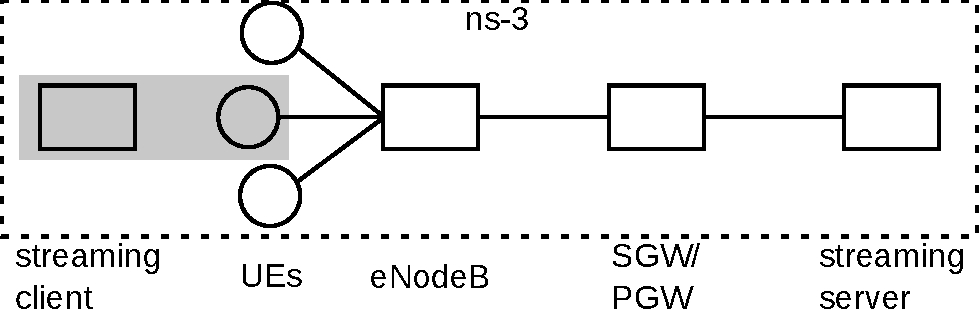
\includegraphics[width=0.6\textwidth]{images/streaming-simulation.pdf}
\caption{\gls{LTE} reliable streaming simulation testebd.}
\label{c5:fig:streaming-simulation}
\end{figure}

\begin{figure}[htb]
\centering
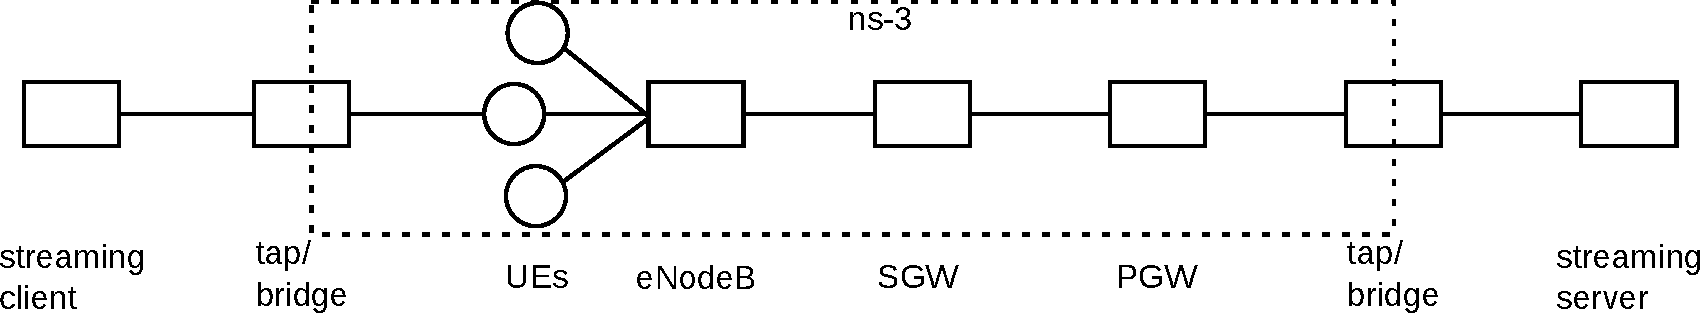
\includegraphics[width=\textwidth]{images/streaming-hybrid.pdf}
\caption{Future testbed iteration: hybrid of ns-3 LTE simulation and actual or emulated streaming client and server bridged to it.}
\label{c5:fig:streaming-hybrid}
\end{figure}

% \begin{figure}[htb]
% \centering
% 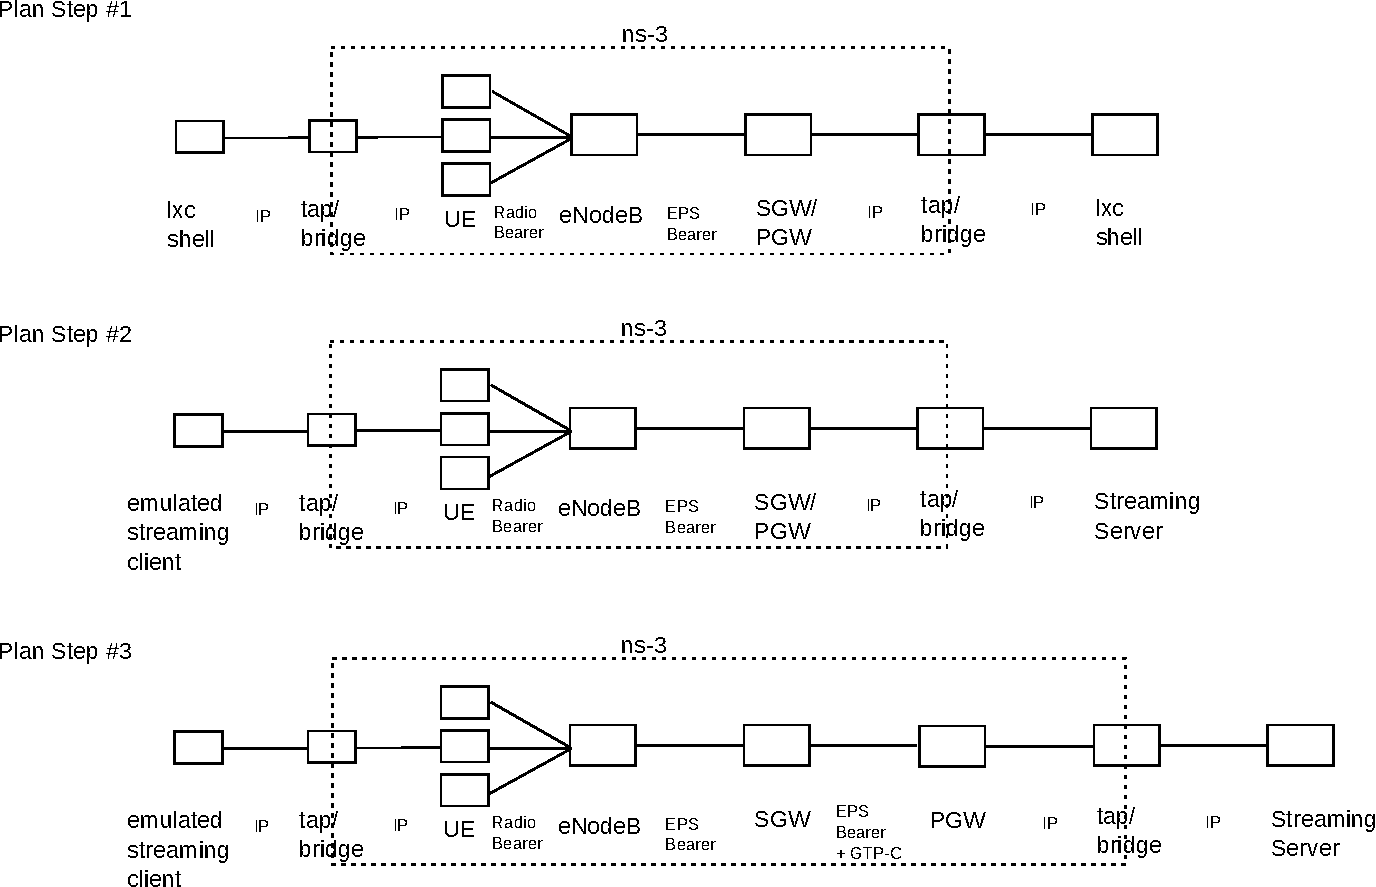
\includegraphics[width=\textwidth]{images/lte-testbed.pdf}
% \caption{\gls{LTE} Streaming Evaluation Setup and Action Plan}
% \label{fig:lte-testbed}
% \end{figure}


%%%%%%%%%%%%%%%%%%%%%%%%%%%%%%%%%%%%%%%%%%%%%%%%%%%%%%%%%%%%%%%%%%%%%%%%%%%%%%%%
\subsubsection{Combined Simulating Streaming Traffic Characteristics in ns-3}
\label{c5:mobilestreamingtestbed}

Different Approaches



Implement a Reliable Streaming Traffic Generator ns-3 Application and a streaming receiver client application.

Describe Streaming Simulation Model and Variables

Describe ns-3/LENA implementation

 Use LENA to transport streams



